\chapter{Evaluation}\label{cha:Evaluation}
Section \ref{sec:results} of this chapter presents the results of the experiment using the proposed approach. Finally, in section \ref{sec:validate}, we validated the synthetically generated images by training a CNN-based disease detection model.

% ✅✅✅✅

\section{Results of generate images}\label{sec:results}
Every image in the 513 diseased leaf collection was overlaid on the 463 sugar beet images for the experiment. As a result of the experiment, 237 520 synthetic images were created. Figure \ref{fig:my_gen_6} and \ref{fig:my_gen_7} are random images from the generated dataset. The generated images are labelled according to their corresponding number in the original image path to easily find the original images used to form the synthetic image. An image could be name for example $cgls\_445\_sb\_342.png$. $Cgls\_445$ is short for disease image number 445 in corn's grey leaf spot image folder, while $sb\_342$ correlates to sugar beet image number 342.

\begin{figure}[!htb]
    \centering
    % 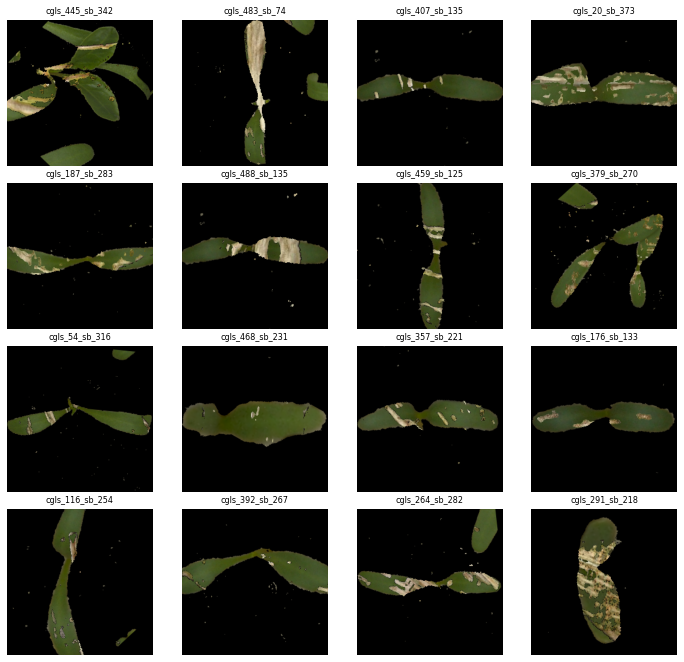
\includegraphics[scale=0.51, keepaspectratio]{Figures/notebook/gen-11.png}
    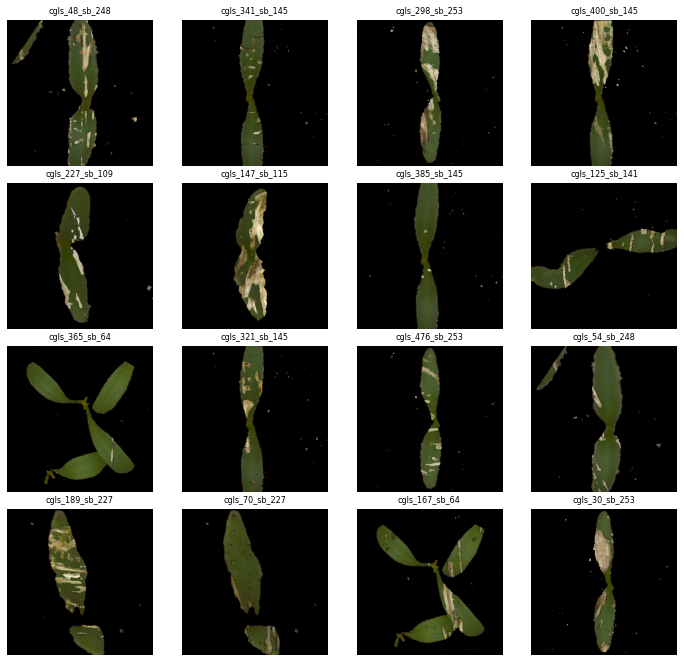
\includegraphics[scale=0.49, keepaspectratio]{Figures/notebook/gen-15.png}
    \caption{Random images from the synthetically generated datasets.}
    \label{fig:my_gen_6}
\end{figure} 

\begin{figure}[!htb]
    \centering
    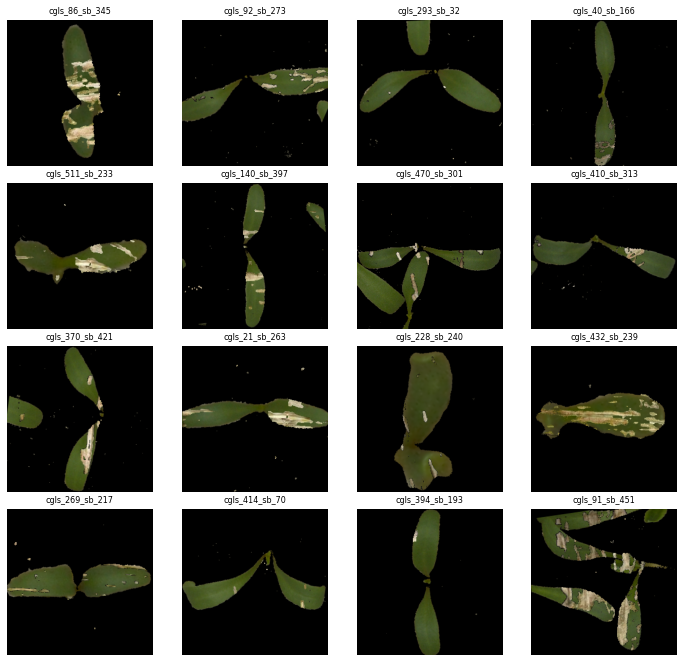
\includegraphics[scale=0.68, keepaspectratio]{Figures/notebook/gen-12.png}
    \caption{Random images from the synthetically generated datasets.}
    \label{fig:my_gen_7}
\end{figure} 

% ✅✅✅
\FloatBarrier
\section{Validation}\label{sec:validate}
CNN-based model training was performed using the generated dataset and the original healthy sugar beet images dataset to validate the generated dataset's efficacy. Four sets of datasets were created for training. The first dataset contains the complete synthetically generated and healthy sugar beet image data. Nine hundred eighty-five randomly chosen synthetic images and all healthy sugar beet images comprise the second dataset. The third dataset consists of 463 synthetic images and 417 healthy sugar beet images. The fourth dataset comprises 453 healthy sugar beet plant images that were not used in synthetic data generation and 1000 synthetically generated images from 10 random sugar beet and 100 random disease plant images.
% The healthy sugar beet images in the four datasets were 
The background of the healthy sugar beet images was segmented across all datasets to avoid the neural network from learning only to make predictions based on the background. Likewise, random image augmentation techniques like random flipping and clipping were used during model training to avoid the problem of overfitting.
The pre-trained versions of Alexnet ResNet 34 and 152 CNN architectures were used for model training to classify input images as healthy or diseased.

Table \ref{table:accuracy} shows the average training time per epoch and accuracy of each architecture trained on the four datasets for five epochs except datasets 2 and 4, which were trained for ten epochs. Models trained on the first dataset had the highest accuracy, which is understandable because of the wide gap between the datasets in the healthy and diseased plant images. The average accuracy of the models across all datasets was above 90\%, which shows the success of the synthetically generated dataset for training disease detection models.

\begin{table}[H]
\centering 
 \begin{tabular}{p{5cm}|c|c|c} 
%   \begin{tabular}{|c|c|c|c|c|}
 \hline
  Dataset & Architecture  & Training time per epoch & Accuracy \\ [0.5ex] 
 \hline
 & ResNet-34 & 6 min 7 s & 100\%  \\ 
 
 Dataset 1 (237, 982 images) & ResNet-152 & 2 min 5 s&99.98\% \\ 
 
 & AlexNet & 33 min 29 s&99.99\% \\ 
 \hline
%  ✅✅✅
 \hline
 & ResNet-34 & 5 s & 93.05\%  \\ 
 
 Dataset 2 (1448 images) & AlexNet & 3 s & 90.27\% \\ 
 
 & ResNet-152 & 31 s & 97.91\% \\ 
 \hline
 %  ✅✅✅
 \hline
 & ResNet-34 & 6 s & 93.75\%  \\ 
 
 Dataset 3 (880 images) & AlexNet & 4 s & 94.88\% \\ 
 
 & ResNet-152 & 18 s & 91.47\% \\ 
 \hline
 %  ✅✅✅
 \hline
 & ResNet-34 & 5 s & 98.62\%  \\ 
 
 Dataset 4 (1453 images) & AlexNet & 4 s & 93.10\% \\ 
 
 & ResNet-152 & 15 s & 98.27\% \\ 
 \hline
 \end{tabular}
 \caption{Accuracies and training time of CNN models trained of four different sets of data.}
 \label{table:accuracy}
\end{table}

